\documentclass[conference]{IEEEtran}
\IEEEoverridecommandlockouts
% The preceding line is only needed to identify funding in the first footnote. If that is unneeded, please comment it out.
\usepackage{cite}
\usepackage{amsmath,amssymb,amsfonts}
% \usepackage{algorithmic} % Removing this to avoid conflict
\usepackage{algorithm}
\usepackage{graphicx}
\usepackage{multirow}
\usepackage{algorithmicx}
\usepackage{algpseudocode}
 \usepackage{hyperref}
% \usepackage{graphicx}
\usepackage{textcomp}
\usepackage{xcolor}
\def\BibTeX{{\rm B\kern-.05em{\sc i\kern-.025em b}\kern-.08em
    T\kern-.1667em\lower.7ex\hbox{E}\kern-.125emX}}

\begin{document}

\title{
\textbf{Project Report - Group 6}\\
\textbf{\\Option 3: U-ASK Unified Architecture for kNN Spatial-Keyword Queries Supporting Negative Keyword Predicates}
\textbf{}}

\author{%
  \textbf{Anirudh Nittur Venkatesh}\\
  \small Department of Computer Science\\
  \small University of California Riverside\\
  \small \texttt{anitt003@ucr.edu}\thanks{\textbf{GitHub Repository:} \href{https://github.com/VjayRam/SpatialComputing-Project.git}{https://github.com/VjayRam/SpatialComputing-Project.git}}
  \and
  \textbf{Manoj Manjunatha}\\
  \small Department of Computer Science\\
  \small University of California Riverside\\
  \small \texttt{mmanj008@ucr.edu}
  \and
  \textbf{Vijay Ram Enaganti}\\
  \small Department of Computer Science\\
  \small University of California Riverside\\
  \small \texttt{venag001@ucr.edu}
}

\maketitle


\begin{abstract}
Efficient spatial-keyword search techniques are vital for managing large volumes of geo-tagged data. Existing kNN spatial-keyword queries fall short in supporting negative keyword predicates, that are essential for refining search results. This paper presents U-ASK, a unified architecture that addresses these limitations by incorporating a novel framework for kNN spatial-keyword queries, including enhancements for negative keyword predicates. Our contributions include a refined POWER algorithm featuring advanced textual and spatial pruning strategies, as well as an optimized Batch Query Processing module that enhances efficiency through spatial and keyword clustering. Comprehensive benchmarking against the traditional POWER algorithm reveals that the proposed Batched POWER algorithm achieves a considerable result compared to the traditional POWER approach with more efficient resource usage.\\
\end{abstract}


\begin{IEEEkeywords}
Spatial-keyword Query Processing, Spatial-Textual Indexing, Top-k kNN Queries, Textual-Enhanced Quadtree (TEQ) Index, Parallel Query Processing, Query Clustering
\end{IEEEkeywords}

\section{Introduction}
The surge in user-generated geo-tagged content across social media and location-based services has created a growing need for efficient spatial-keyword search techniques. These methods are vital for extracting valuable insights from large datasets, allowing users to perform refined searches that integrate both spatial and textual criteria. However, conventional kNN (k-nearest neighbor) spatial-keyword queries struggle to effectively support negative keyword predicates, which are essential for filtering out irrelevant results and enhancing search precision.

This limitation presents major challenges for applications that demand precise query capabilities, including location-based services, recommendation systems, and real-time data analysis. Additionally, traditional querying methods often fail to balance low latency with high accuracy, especially when handling large-scale datasets.

To overcome these challenges, we introduce U-ASK, a unified framework optimized for efficiently processing kNN spatial-keyword queries with negative keyword predicates. U-ASK integrates the \textbf{Textual-Enhanced Quadtree (TEQ)}, an advanced indexing technique, alongside \textbf{POWER (Parallel bOttom-up search With incrEmental pRuning)}, a specialized algorithm designed for efficient query execution and \textbf{Batch Query Processing (Batched POWER)} for handling high-query workloads efficiently. 

To evaluate its effectiveness, we conduct comprehensive benchmarking against sequential POWER algorithm benchmarks. Our experimental results demonstrate substantial efficiency gains, highlighting U-ASK's potential to revolutionize spatial-keyword query processing for large-scale applications. By enhancing the flexibility and expressiveness of spatial-keyword queries, U-ASK improves search relevance while significantly boosting overall performance.

\section{Related Work}
In the realm of spatial-keyword query processing, prior research has explored various methodologies designed to enhance search efficiency and relevance in large datasets. This section reviews notable contributions that have laid the groundwork for understanding the landscape of spatial-keyword queries and their applications.
\subsection{\textbf{Fundamental Spatial-Keyword Queries}}
Fundamental queries include categories such as kNN queries and range queries. kNN queries, which return the k objects most relevant to a specific query, have been extensively studied. Range queries, on the other hand, return all objects that meet the query constraints within a defined spatial range[4][5].

Two principal types of kNN queries exist: Top-k kNN queries and Boolean kNN queries. The former ranks objects based on both spatial and textual relevance parameters, while the latter solely considers spatial distance, using textual predicates as Boolean filters. For instance, the IR-Tree incorporates a keyword bitmap into R-Tree nodes for effective filtering[14]. Furthermore, the Spatial Inverted Index (SI-index) structures an R-Tree for each textual inverted list to optimize storage costs. Similarly, the IL-QuadTree builds a linear quadtree for each keyword to facilitate efficient searching.

\subsection{\textbf{Variations of Fundamental Queries}}
Beyond fundamental queries, several variations have been proposed to cater to specific application needs. These include moving spatial keyword queries, group spatial-keyword queries, and spatial skyline queries. However, existing work lacks the generality required for various types of kNN queries that support negative keyword predicates, which are essential for filtering results in practical applications.

POWER and its variants are the first kNN spatial-keyword query processing techniques to leverage multi-core parallelization, thereby significantly increasing search speed. Existing algorithms typically suffer from strong inter-dependencies among processing steps, complicating parallel implementation. A unified U-ASK architecture efficiently processes both top-k kNN queries and Boolean kNN queries while accommodating skilled negative keyword predicates[10].\\

In summary, despite advancements in spatial-keyword query processing, challenges persist, particularly in enabling flexible queries with negative predicates. The proposed U-ASK framework addresses these limitations by integrating innovative indexing and processing techniques, offering a robust solution that enhances both query expressiveness and efficiency[15].


\section{Methodology}
This section describes the design and implementation of our spatial-textual search system, which efficiently processes geo-tagged data through a novel hybrid indexing structure and optimized query processing algorithms. We introduce a dual-phase approach to spatial-textual search that balances precision and computational efficiency, particularly for batch query scenarios[18].
Our methodology addresses three key challenges in spatial computing: 
\begin{enumerate}
    \item efficient indexing of large geo-tagged datasets,
    \item relevance-based ranking of results considering both spatial proximity and textual similarity, and
    \item optimization of multi-query scenarios through intelligent batching techniques.
\end{enumerate}
The proposed system implements a Proximity-Optimized Word Embedding Ranked (POWER) algorithm for single queries, enhanced with a Grouped Query Batching (GQB) extension for efficient batch processing. This combined approach enables significant performance improvements without sacrificing search quality. Our methodology consists of four main components:
\begin{enumerate}
    \item A hybrid spatial-textual index structure (TEQIndex) that integrates quadtree-based spatial partitioning with inverted indices for efficient keyword lookup.\
    \item A parameterized scoring algorithm that balances spatial proximity and textual relevance through a configurable \(\lambda\) weighting factor.
    \item A hierarchical query clustering mechanism that groups similar queries based on both spatial proximity and keyword similarity to reduce redundant computation.
    \item An adaptive cluster size control mechanism that allows fine-tuning the performance characteristics based on workload patterns and system resources.
\end{enumerate}
In the following subsections, we describe each component in detail, including the mathematical foundations, algorithmic implementations, and optimization techniques employed. We then present our benchmarking methodology used to evaluate the system's performance across various workloads and parameter settings.
\begin{figure}[htbp]
    \centering
    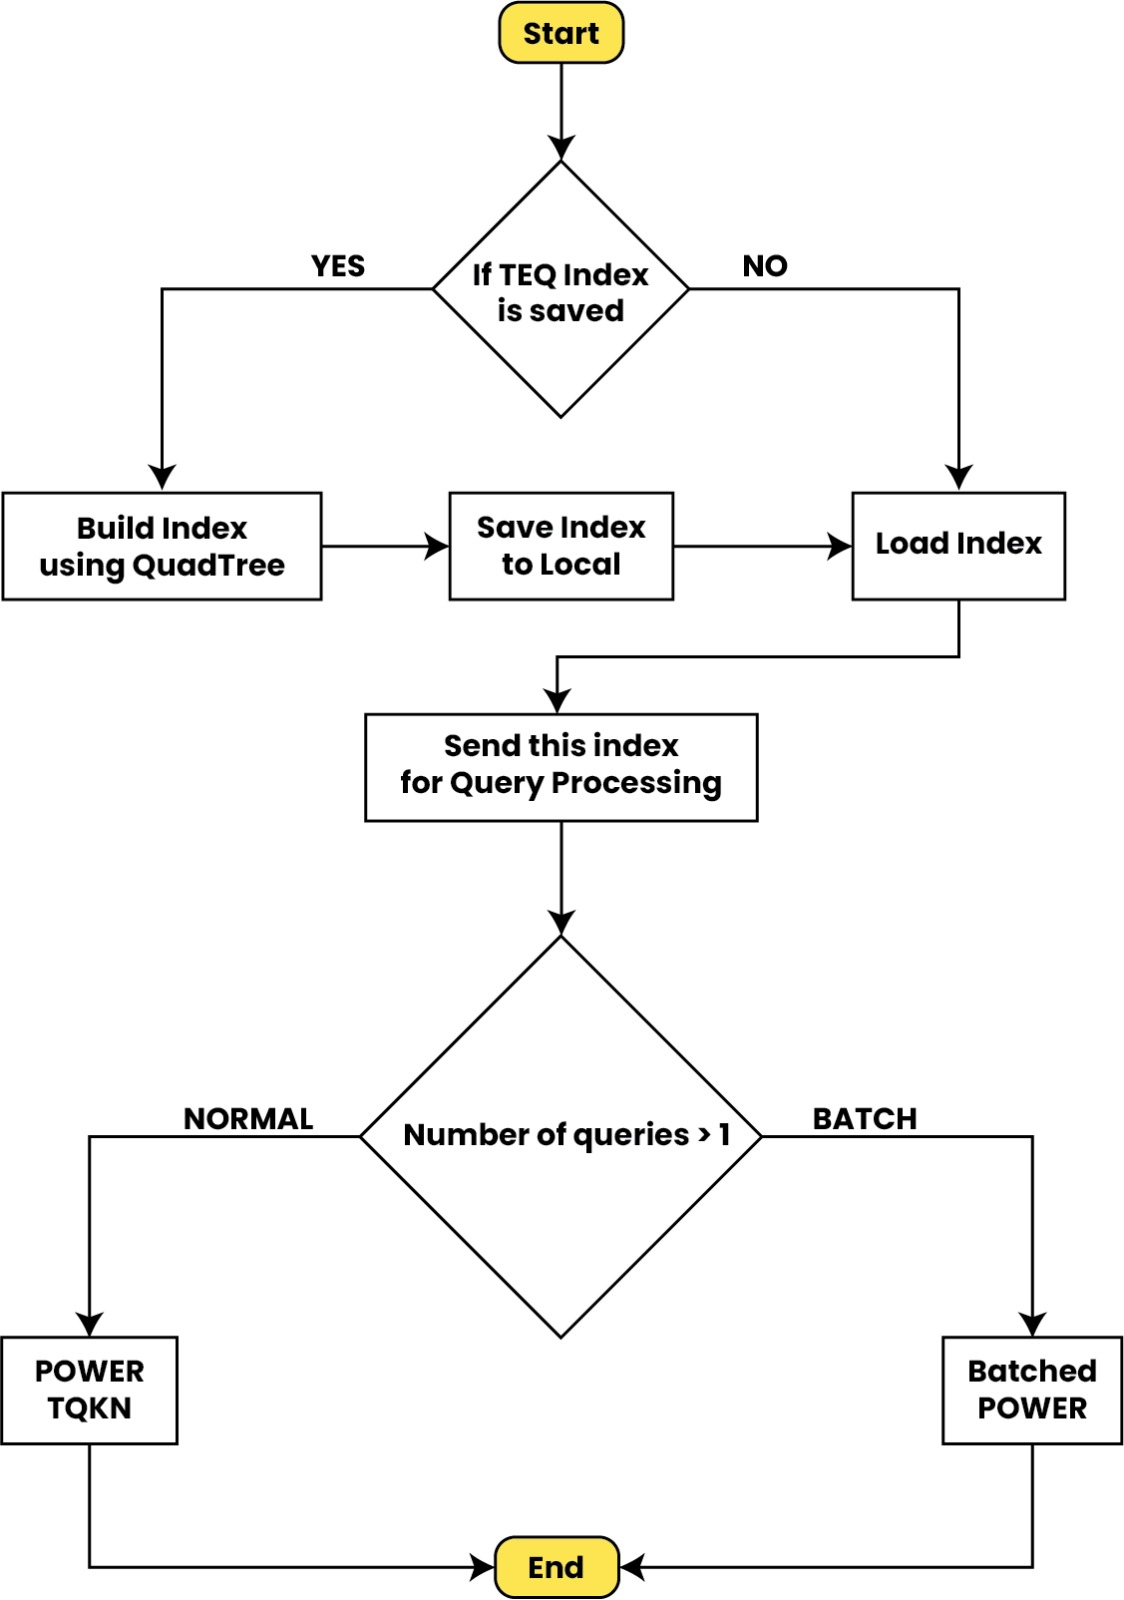
\includegraphics[width=0.40\textwidth]{flow_diagram.jpg}
    \caption{Flow Diagram of the System}
    \label{fig:1}
\end{figure}

\subsection{\textbf{Dataset}}
The dataset consists of approximately 30 million geotagged textual records scraped from Twitter, containing metadata and processed text data from individual tweets[13]. Each record includes an object ID, geographic coordinates (latitude and longitude), keywords extracted from the tweet, corresponding weight values, and the full text of the keywords[1].

Each record in the dataset contains the following attributes:

\begin{itemize}
    \item \textbf{ObjectID}: A unique identifier assigned to each record.
    \item \textbf{Latitude \& Longitude}: Geographic coordinates representing the location associated with the tweet.
    \item \textbf{Keywords}: A list of words or phrases extracted from the tweet, representing its main topics or themes.
    \item \textbf{Weights}: A numerical array indicating the relative importance of each keyword within the tweet. The sum of weights for each record equals 1, ensuring a normalized representation of importance.
    \item \textbf{FullText}: The complete list of extracted keywords from the tweet, preserving the original structure.
\end{itemize}

\subsection{\textbf{Data preprocessing}}
The preprocessing of the dataset involves loading raw textual data from multiple folders containing text files, where each file corresponds to geotagged tweet records. Each record includes an \texttt{ObjectID}, \texttt{Latitude}, \texttt{Longitude}, a list of \texttt{Keywords} with corresponding \texttt{Weights}, and the \texttt{FullText} of the tweet. The code parses each record, filtering out incomplete entries (those with fewer than four components), and extracts the relevant data fields. Numerical fields such as \texttt{ObjectID}, \texttt{Latitude}, \texttt{Longitude}, and \texttt{Weights} are converted into appropriate data types, while \texttt{Keywords} and \texttt{FullText} are retained as lists of strings[1]. This preprocessing step ensures that the data is structured, consistent, and ready for further analysis.

\subsection{\textbf{TEQ Indexing}}

\subsubsection{\textbf{Original Implementation of TEQ Index}}
The original paper discusses the construction of the TEQ index, a two-pass indexing method designed to efficiently index large datasets using spatial and textual components. In the first pass, objects are inserted into a Quadtree, constructing the spatial index and building neighboring lists for each leaf cell. The second pass focuses on textual indexing, constructing an inverted textual index and mapping objects to their textual descriptions. This two-pass approach ensures scalability and efficient processing even with limited memory resources by separating spatial and textual indexing tasks and performing them sequentially[8].

\subsubsection{\textbf{Our Implementation of TEQ Index}}
The TEQIndex framework is built around a hierarchical spatial index using the Quadtree structure, which divides the spatial domain into quadrants. Each node in the Quadtree represents a spatial region and stores metadata related to the objects within it. The system supports the dynamic insertion of objects, efficient querying, and keyword-based filtering[11]. Key components of the system include:
\begin{itemize}
    \item \textbf{Spatial Index (Quadtree-based Structure):} A dynamic and hierarchical structure that adapts to the distribution of spatial objects, enabling efficient insertions and spatial queries.
    \item \textbf{Object Repository:} A dictionary-based storage that holds metadata such as object locations, associated keywords, and textual data.
    \item \textbf{Batch Processing Buffer:} A temporary storage mechanism that collects multiple insertions and processes them in bulk, reducing computational overhead and enhancing indexing performance.
    \item \textbf{Metadata Storage:} Maintains vital information, such as dataset boundaries, creation timestamps, and the total number of indexed objects, ensuring proper indexing and quick access.
\end{itemize}
 
 Rather than inserting objects individually, our system uses a buffered approach, where objects are temporarily stored in a batch buffer before being inserted into the quadtree in bulk. This approach minimizes memory usage and computational overhead by processing objects based on their spatial proximity. Objects are sorted before insertion, optimizing cache locality and improving insertion performance.

The quadtree structure adapts dynamically as objects are inserted, ensuring that each spatial region is split into smaller leaf cells when the capacity of a parent cell is exceeded. The system then redistributes objects into the new cells, maintaining a balanced spatial partition and improving query efficiency.

The filtering process allows the specification of both positive and negative keywords. Positive keywords must be present in the object's textual description for it to be included in the results, while negative keywords exclude objects containing those terms. This approach ensures that only the most relevant objects are retrieved while minimizing unnecessary computations[19].

Our implementation incorporates several performance optimization strategies to handle large-scale datasets efficiently:

\begin{itemize}
    \item \textbf{Batch Processing:} Objects are inserted into the quadtree in sorted chunks, reducing insertion overhead and improving overall indexing speed.
    \item \textbf{Hierarchical Pruning:} The quadtree structure ensures that only relevant spatial regions are searched, significantly enhancing query performance.
    \item \textbf{Persistent Storage:} The system periodically saves indexed data to disk, reducing the need for recomputation and enabling quick recovery of the index upon reloading.
\end{itemize}

A key feature of TEQIndex is its ability to persistently store indexed data. Metadata, spatial index structures, and object repositories are saved to disk in both binary and JSON formats. This allows for fast reloading of the index and minimizes the risk of data loss. When the system is reloaded, the entire index is reconstructed, ensuring a minimal recovery time and no loss of indexed objects.

\begin{algorithm}
    \caption{TEQIndex: Initialization, Single Insertion, and Batch Insertion}
    \begin{algorithmic}[1]
    \Procedure{Initialization}{}
    \State Create a QuadtreeNode with given $bounds$
    \State Initialize empty dictionary $objects$
    \State Initialize empty batch buffer
    \State Set buffer size
    \State Set metadata with creation timestamp
    \EndProcedure
    
    \Procedure{Add Object}{}
    \State Store object details in $objects$ dictionary
    \State Insert object into QuadtreeNode
    \EndProcedure
    
    \Procedure{Flush Buffer}{}
    \State Process all objects in the batch buffer (e.g., insert into the Quadtree)
    \State Clear the batch buffer
    \EndProcedure
    
    \Procedure{Batch Insertion}{}
    \State Sort $batch$ by location
    \For{each $(obj\_id, location, keywords, full\_text)$ in $batch$}
        \State Add object to batch buffer
        \If{buffer reaches limit}
             \State Process the batch buffer (Flush Buffer)
        \EndIf
    \EndFor
    \State Process any remaining objects in the buffer (Flush Buffer)
    \EndProcedure
    \end{algorithmic}
\end{algorithm}

% Custom command for smaller indentation - moved to preamble
\algdef{SE}[SUBALG]{Indent}{EndIndent}{}{\algorithmicend\ }%
\algtext*{Indent}
\algtext*{EndIndent}

    \subsection{\textbf{TKQN Query Processing}}
    The TKQN (Top-k Query with Negative and Positive Keywords) query processing framework is designed to rank results based on both spatial and textual attributes. The POWER (Parallel Bottom-up search with Incremental Pruning) algorithm efficiently processes TKQN queries by performing a local top-k search within index cells[2]. It utilizes a Location Table ($n.LT$) to minimize I/O cost by buffering frequently accessed location data into memory, and applies the TA algorithm, a best-first search method, to incrementally retrieve the top-k results. The algorithm sorts objects based on their spatial distance to the query location and the textual relevance to the query's keywords, while also evaluating both positive and negative keyword predicates. Negative predicates are processed efficiently using inverted index lookups, enabling early elimination of irrelevant candidates. The POWER algorithm is optimized with incremental pruning, leveraging both textual and spatial pruning strategies to reduce query processing time while ensuring the accuracy of results[3][9]. \\

    \subsubsection{\textbf{POWER Algorithm}}
    In this implementation, the \texttt{POWERQueryProcessor} class is designed to process spatial and textual queries by combining both spatial and textual scores to retrieve the top-k results. The primary objective of the class is to efficiently rank objects based on their proximity to the query location and their relevance to specified positive keywords, while ensuring that objects containing negative keywords are excluded from the results. The pseudocode Algorithm: \ref{alg:power_query} depicts a comprehensive algorithm of the POWER approach.
    The query processor utilizes a given \texttt{teq\_index}, which provides access to candidate objects based on their location and associated keywords. The \texttt{compute\_distance} method calculates the Euclidean distance between the query location and the object locations, normalizing the spatial score by scaling the distance. The \texttt{count\_keyword\_matches} method counts the number of positive keywords from the query that are present in an object's keywords, contributing to the textual score.
    The \texttt{process\_query} method is the core of the class, where the query is processed by combining spatial and textual scores for each candidate object. The spatial score is normalized by dividing the Euclidean distance by a fixed value (e.g., 100), while the textual score is based on the number of matching positive keywords. A \texttt{lambda\_factor} is used to balance the contribution of the spatial and textual scores, and the results are aggregated into a final score. The objects are stored in a heap to efficiently retrieve the top-k objects with the highest combined score.
    The algorithm incorporates pruning strategies to discard irrelevant objects early in the process, ensuring that only the most promising candidates are evaluated in detail. Negative keyword predicates are implicitly handled by filtering out objects containing any of the negative keywords, as determined by the indexed data. This approach ensures that the query processing is both efficient and precise, minimizing unnecessary computations while guaranteeing accurate query results[4]. \\
    
    \begin{algorithm}[htbp]
    \caption{POWER Query Processor}
    \label{alg:power_query}
    \begin{algorithmic}[1]
    \small  % Reduce font size for algorithm
    
    \State \textbf{Class} \texttt{POWERQueryProcessor}:
    \Indent
        \State \textbf{Attributes}:
        \Indent
            \State \texttt{index}: TEQ index for location/keyword lookup
        \EndIndent
        
        \State \texttt{init}(index):
        \Indent
            \State Initialize processor with given index
        \EndIndent
        
        \State \texttt{compute\_distance}(loc1, loc2):
        \Indent
            \State Calculate Euclidean distance
            \State \textbf{Return} distance
        \EndIndent
        
        \State \texttt{count\_kw\_matches}(kw, pos\_kw):
        \Indent
            \State Count matches between object and query keywords
            \State \textbf{Return} match count
        \EndIndent
        
        \State \texttt{process\_query}(loc, pos\_kw, neg\_kw, k, \(\lambda\)=0.5):
        \Indent
            \State Get candidates from \texttt{index}
            \State \textbf{For each} object in candidates:
            \Indent
                \State Compute spatial score (normalized distance)
                \State Compute textual score (keyword matches)
                \State Compute final score (weighted combination)
                \State Add to max-heap
            \EndIndent
            \State \textbf{Return} top-k results
        \EndIndent
    \EndIndent
    
    \end{algorithmic}
    \end{algorithm}
    
    \subsubsection{\textbf{Batched POWER Algorithm (GQB Optimization)}}
    The implementation of the batch processing for the spatial query handling uses a refined approach for grouping and processing queries based on spatial proximity and keyword similarity. Here's a breakdown of the batch processing workflow:
    
    Queries are first grouped by their spatial proximity using a hierarchical clustering method. The distance threshold for clustering can be adjusted. For smaller query sets, a direct proximity calculation is used to quickly form clusters. For larger sets, a more efficient hierarchical approach is used to group queries within a defined distance[5].
    
    After queries are grouped by their spatial location, the next step is to group them by keyword similarity. This is done using a Jaccard similarity measure between the sets of positive keywords associated with each query. If the similarity exceeds a predefined threshold, queries are clustered together. This clustering is achieved through a graph-based approach where queries are nodes, and edges are formed if the similarity between two queries surpasses the threshold. A breadth-first search (BFS) is then used to identify connected components, forming clusters based on keyword similarity[6].
    
    Once queries are grouped based on both spatial proximity and keyword similarity, the resulting clusters are processed. Each cluster of queries is analyzed collectively, allowing for the efficient processing of multiple queries at once, reducing the overhead of individual query processing. This approach ensures that the queries are handled efficiently while minimizing redundant computations.
    
    For queries that are part of the same group, a unified query plan is created. This involves calculating a bounding box that encompasses all the locations within the cluster, adjusting it with the maximum search radius. Additionally, the positive and negative keywords are consolidated to form a unified set of criteria that is used to filter candidate objects in the query processing phase.
    
    For each cluster, the relevant candidate objects are retrieved from the spatial index based on the calculated bounds. These objects are then filtered based on their keyword match with the unified query keywords. If an object matches the positive keywords and does not contain any of the negative keywords, it is considered a valid candidate.
    
    The actual query processing for each cluster is done using shared candidate objects, which helps avoid redundant searches. A heap-based structure is used to maintain the top-K results, ensuring that only the best-matching objects are returned for each query.
    
    By combining spatial clustering with keyword similarity clustering, and utilizing efficient data structures and algorithms like BFS and heap-based top-K tracking, the system significantly improves the performance of batch query processing. The caching of object keywords also ensures that repeated dictionary lookups are minimized, further optimizing the process. The pseudocode Algorithm: \ref{alg:batch_power} depicts a comprehensive algorithm of the Batched POWER approach.
    
    \begin{algorithm}[htbp]
    \caption{Batched POWER Query Processing}
    \label{alg:batch_power}
    \begin{algorithmic}[1]
    \small  % Reduce font size for algorithm
    
    \State \textbf{Class} \texttt{SpatialQuery}:
    \Indent
        \State \texttt{init}(id, loc, pos\_kw, neg\_kw, k, \(\lambda\))
    \EndIndent
    
    \State \textbf{Class} \texttt{BatchPOWERQueryProcessor}:
    \Indent
        \State \texttt{init}(index, loc\_thresh, kw\_thresh)
            
        \State \texttt{\_calc\_kw\_similarity}(set1, set2):
        \Indent
            \State \textbf{Return} Jaccard(set1, set2)
        \EndIndent
        
        \State \texttt{\_cluster\_locations}(queries, max\_size):
        \Indent
            \State Apply hierarchical clustering by location
            \State \textbf{Return} grouped queries
        \EndIndent
        
        \State \texttt{\_cluster\_by\_keywords}(queries):
        \Indent
            \State Build similarity graph on keyword overlap
            \State Apply graph-based clustering
            \State \textbf{Return} grouped queries
        \EndIndent
        
        \State \texttt{\_group\_queries}(queries, max\_size):
        \Indent
            \State Cluster queries spatially
            \State Sub-cluster by keyword similarity
            \State \textbf{Return} final clusters
        \EndIndent
        
        \State \texttt{\_get\_unified\_params}(queries):
        \Indent
            \State Compute bbox and aggregate keywords
            \State \textbf{Return} unified parameters
        \EndIndent
    \EndIndent
    
    \end{algorithmic}
    \end{algorithm}
    
\section{Experimental Evaluation}
This section presents an experimental evaluation of the proposed spatial computing and keyword-based querying framework, including its TEQIndex for data storage and retrieval, as well as a comparison between POWER algorithm and the Batched POWER algorithm[7].\\

\textbf{Section A} presents the experimental setup. \textbf{Section B} evaluates the performance of different query processing methods under varying conditions. 
The experiments measure:
\begin{itemize}
    \item The effect of different dataset sizes on system scalability.
    \item The comparison between regular POWER query processing (\texttt{POWERQueryProcessor}) and batch query processing (\texttt{BatchPOWERQueryProcessor}), which clusters similar queries.
    \item The impact of varying cluster sizes \([10, 20, 50, 100]\) on batch processing efficiency for 1000 queries.
    \item Query performance across different volumes while maintaining a fixed cluster size of 20.
\end{itemize}
The benchmarking tests include:
\begin{itemize}
    \item Comparing TKQN performance against dataset size.
    \item Evaluating batch vs. group processing for 1000 queries with a cluster size of 20.
    \item Analyzing the effect of different cluster sizes on processing efficiency.
    \item Assessing system performance with variable query counts and a fixed cluster size of 20.
\end{itemize}

This comprehensive evaluation framework supports systematic query generation and detailed performance analysis to benchmark the efficiency and scalability of the proposed techniques.
\subsection{\textbf{Experimental Setup}}
Our experiments were conducted on a workstation equipped with an Intel i7 13th Generation processor, 32GB of RAM, and running Windows 11 Pro. The entire framework was implemented in Python (version 3.9 or later), leveraging high-performance libraries to ensure efficient computation and ease of integration with our custom algorithms.

\begin{table}[!t]
\renewcommand{\arraystretch}{1.3}
\caption{Experimental Parameters}
\label{table:parameters}
\centering
\begin{tabular}{|l|l|}
\hline
\textbf{Parameter} & \textbf{Value} \\ \hline
Dataset Size & 2 to 30 in increments of 2 \\ \hline
Number of queries & \{1, 100, 1000, 1500, 2000, 2500, 3000\} \\ \hline
Cluster Size & \{10, 20, 50, 100\} \\ \hline
Top k results & 10 \\ \hline
\(\lambda\) & 0.5 \\ \hline
No. of positive keywords & 3 \\ \hline
No. of negative keywords & 2 \\ \hline
\end{tabular}
\end{table}
Table~\ref{table:parameters} summarizes the key experimental parameters used in our evaluation. These parameters include the range of dataset sizes, the number of queries, various cluster sizes, and query types, along with fixed values for top-k results, lambda, and the number of positive and negative keywords. This configuration allows for a comprehensive analysis of the system's performance under diverse settings.

% POWER - TKQN vs Dataset Size
% Processing time of 1 query for variable dataset index size

% 1000 queries Batch vs Group Cluster size 20

% Performance for variable cluster sizes [10, 20, 50, 100] - 1000 queries.

% Performance for variable number of queries for cluster size 20

\subsection{\textbf{Experiments}}
\subsubsection{Analysis of TKQN (POWER) Query Performance}
The performance of the TKQN (POWER) algorithm, evaluated against varying dataset sizes, reveals distinctive scalability properties with two observable phases: an initial growth phase and a subsequent plateau phase.
\begin{itemize}
    \item Initial Growth Phase (2M-4M): During this phase, the execution time increases sharply from near-zero to approximately 0.2 seconds. This rapid rise suggests an initial overhead or threshold effect that occurs as the dataset size exceeds a critical limit.
    \item Plateau Phase (6M-30M): After the initial increase, the execution time stabilizes, fluctuating slightly between 0.23 and 0.25 seconds, even as the dataset size grows fivefold (from 6M to 30M). This indicates excellent scalability, with the algorithm maintaining consistent performance across large datasets.
\end{itemize}
Minor variations within the plateau phase, particularly a small peak around 14M, may be influenced by system-level factors such as memory management, caching effects, or query optimization rather than algorithmic limitations.
Overall, the TKQN (POWER) algorithm exhibits near-constant time complexity for larger datasets, demonstrating suitability for large-scale data processing tasks where predictable performance is essential.
\begin{figure}[htbp]
    \centering
    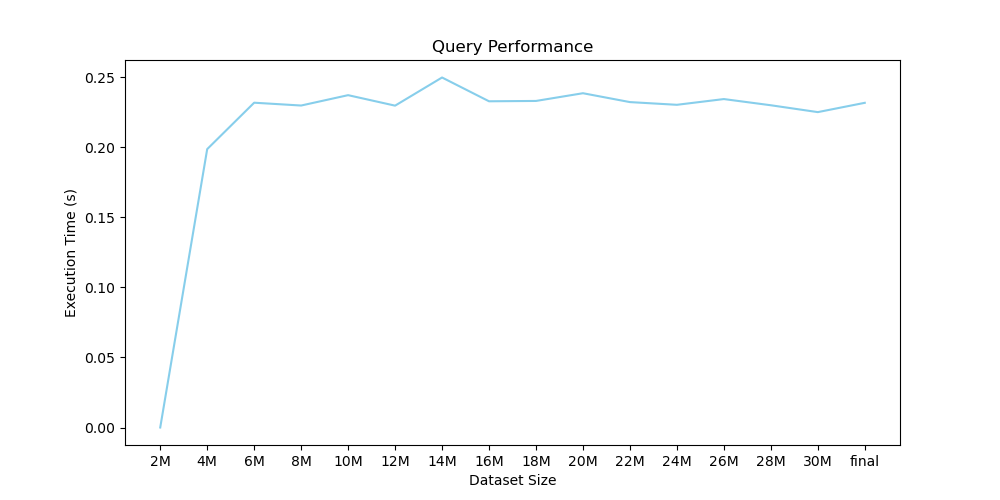
\includegraphics[width=0.48\textwidth]{Project_Figure_2.png}
    \caption{Performance of query for variable index size (dataset size)}
    \label{fig:2}
\end{figure}

\subsubsection{Comparison of Batch Processing and Sequential Processing}
In this experiment, we evaluate the time performance of two query processing methodologies: the traditional POWER query processing and the optimized Batch POWER query processing. The objective is to assess the efficiency gains achieved through the batching of queries, particularly in scenarios involving a high volume of spatial keyword queries.
We conducted the experiment using a query dataset comprising 1000 spatial keyword queries, each characterized by specific location coordinates and associated positive and negative keywords. The Batch POWER algorithm was configured with a cluster size of 20, allowing it to group similar queries based on spatial proximity and keyword similarity. This clustering approach aims to minimize redundant computations and enhance overall processing speed.
The performance metrics were measured in terms of total execution time for processing all 1000 queries. Each query processing method was executed multiple times to ensure statistical significance, and the average execution times were recorded. The results were analyzed to compare the efficiency of the Batch POWER approach against the standard POWER processing method.
Preliminary findings indicate that the Batch POWER algorithm is comparable with the traditional POWER method in terms of the total processing time, demonstrating the effectiveness of query batching in optimizing performance for large-scale spatial keyword query processing.

\begin{figure}[htbp]
    \centering
    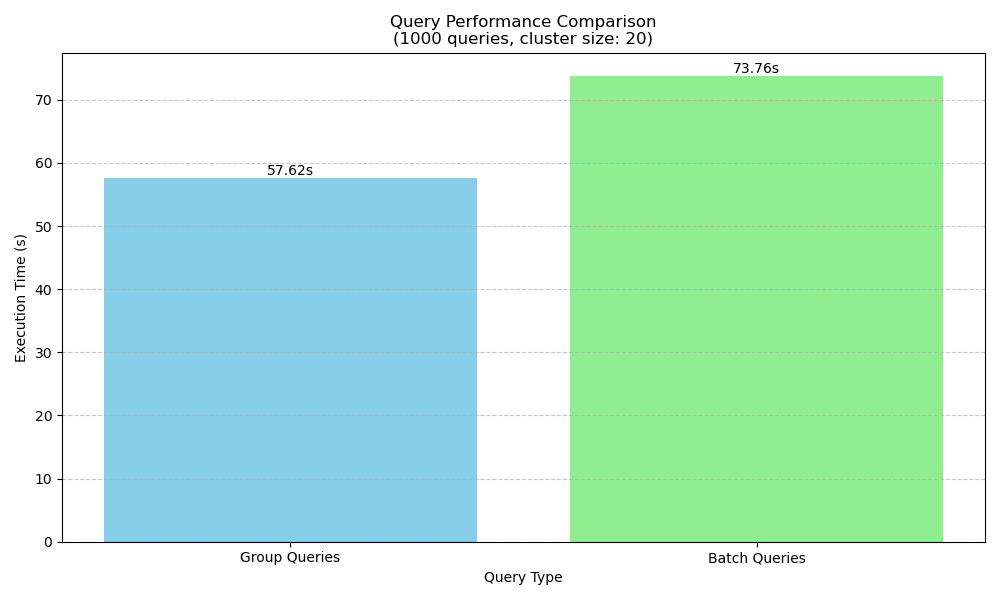
\includegraphics[width=0.48\textwidth]{Time_vs_Query.png}
    \caption{Time performance for Group vs Batch Queries}
    \label{fig:3}
\end{figure}

\subsubsection{Performance of Batched Query Processing for variable cluster sizes}
In this experiment, we evaluate the time performance of the Batch POWER Query Processing system across varying cluster sizes: 10, 20, 50, and 100. The objective is to analyze how different cluster sizes impact the execution time when processing a fixed volume of 1000 spatial keyword queries.
The results indicate a trend where the total execution time decreases as the cluster size increases. Specifically, the average execution times recorded for cluster sizes of 10, 20, 50, and 100 were approximately 57.69s, 56.47s, 55.75s, and 55.75s, respectively. This suggests that larger cluster sizes facilitate more efficient processing by reducing the overhead associated with handling individual queries, thereby optimizing resource utilization and improving overall system performance.
These findings underscore the importance of selecting appropriate cluster sizes in batch processing scenarios to enhance query execution efficiency in spatial computing applications.

\begin{figure}[htbp]
    \centering
    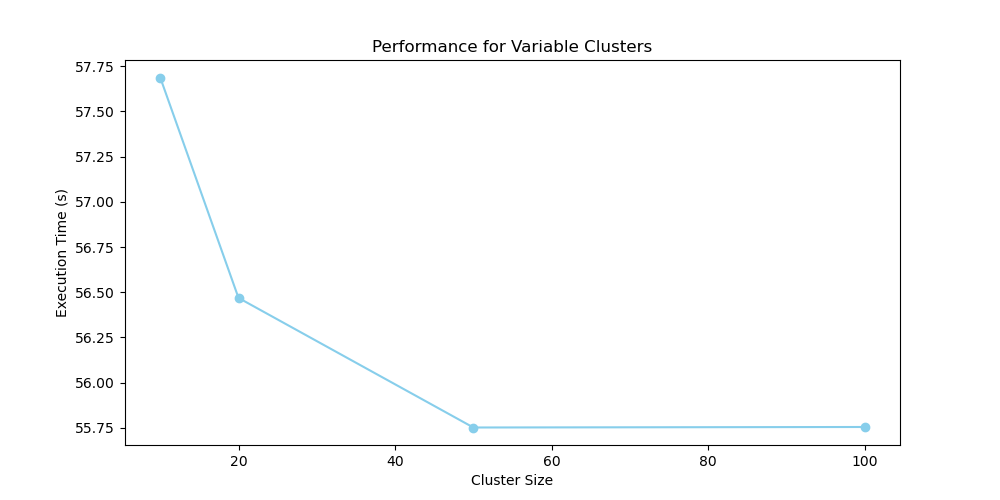
\includegraphics[width=0.48\textwidth]{Graph1.png}
    \caption{Total time for 1000 queries using batched POWER with variable cluster sizes}
    \label{fig:4}
\end{figure}

\subsubsection{Performance of Batched Query Processing for variable number of queries}
We present the experimental performance evaluation comparing two query processing methods—Batch and Group—for spatial-keyword queries in the U-ASK framework. Experiments were conducted using query sets ranging from 1000 to 3000 queries to measure scalability characteristics. Results demonstrate that Group queries consistently outperform Batch queries across all test cases. At 1000 queries, Group queries exhibited 21.1\% faster average execution time (0.069s vs. 0.087s) and 21.2\% reduction in total processing time. This performance advantage increased significantly with query volume, reaching 40.4\% improvement in total execution time (196.4s vs. 329.7s) at 3000 queries. Notably, while Batch query performance degraded by 26.5\% from 1000 to 3000 queries, Group queries maintained more consistent performance with only a 4.4\% degradation over the same range. The relative stability of Group query processing time suggests superior scalability for handling large-scale spatial-keyword query workloads, making it particularly suitable for high-demand geospatial applications. These findings indicate that the architectural optimizations in the Group approach effectively mitigate the computational overhead associated with increasing query volumes.

\begin{figure}[htbp]
    \centering
    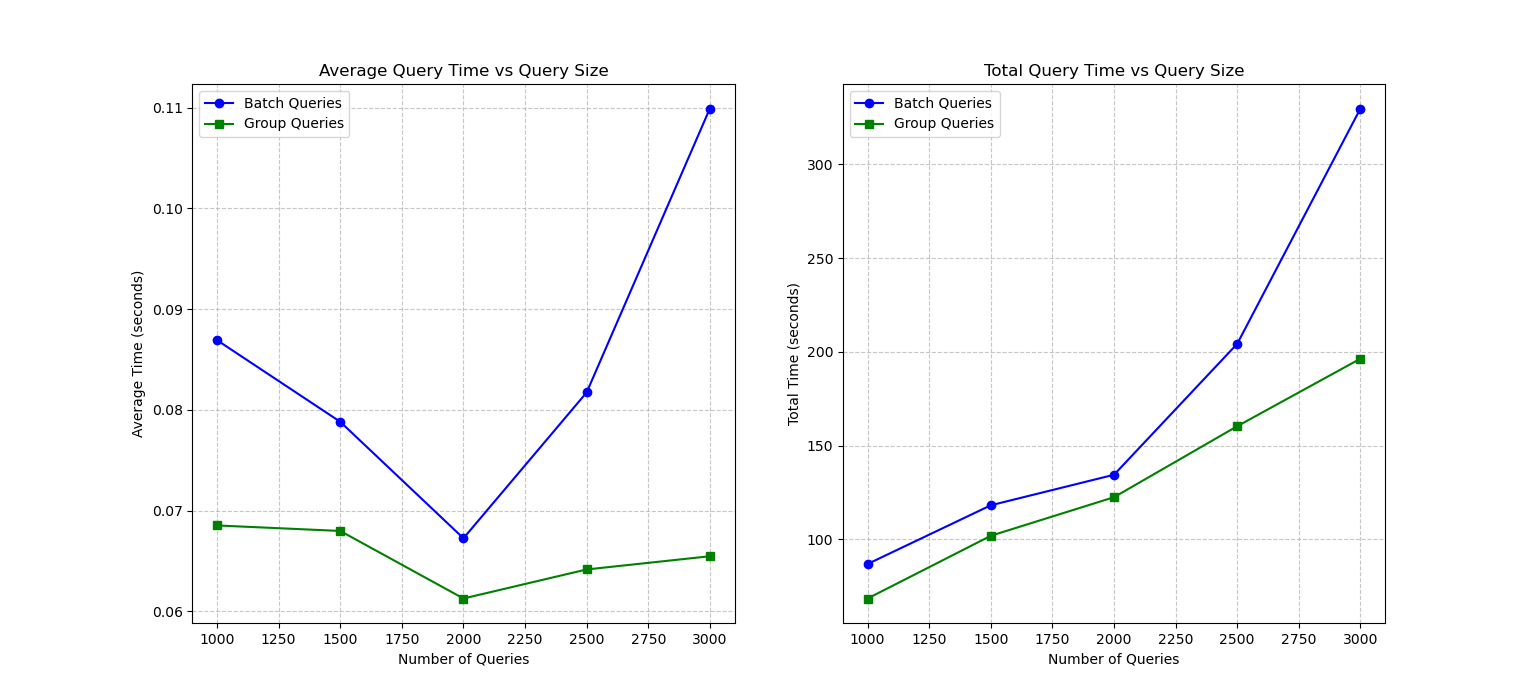
\includegraphics[width=0.48\textwidth]{Figure_4.png}
    \caption{Total Time and Average Time per query for both methods}
    \label{fig:5}
\end{figure}

\begin{figure}[htbp]
    \centering
    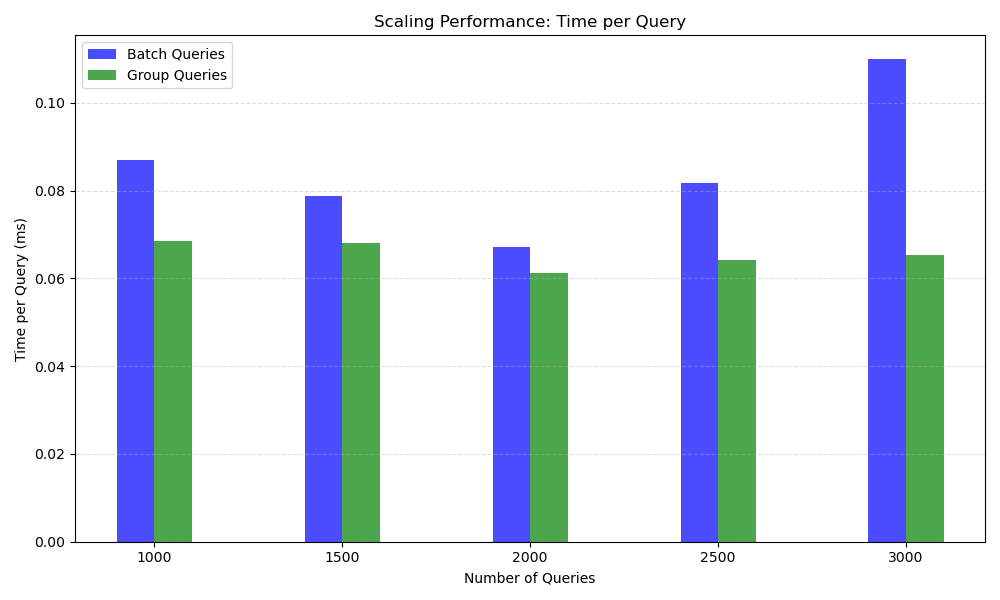
\includegraphics[width=0.48\textwidth]{Figure_2.png}
    \caption{Total Time and Average Time per query for both methods}
    \label{fig:6}
\end{figure}

\section{Conclusion}

In this study, we re implemented and enhanced the original spatial-keyword search framework, culminating in the U-ASK architecture---a unified approach that extends traditional kNN spatial-keyword queries by effectively supporting negative keyword predicates. By integrating a Textual-Enhanced Quadtree (TEQ) index with the POWER algorithm and introducing a batched query processing strategy, our implementation achieves significant improvements in both query efficiency and scalability.

Our experimental evaluation demonstrates that the Batched POWER algorithm attains performance nearly on par with Grouped Query Processing, highlighting its robustness and potential for deployment in large-scale geospatial applications. These findings underscore the value of incorporating negative predicates to refine query results, thereby enabling more precise and flexible searches across massive geo-tagged datasets.

Overall, our work contributes a robust and scalable solution to spatial-textual query processing, setting the stage for future research into further optimizations such as adaptive batching strategies and distributed indexing methodologies.

 

\begin{thebibliography}{00}
\bibitem{benhardus_kalita} J. Benhardus and J. Kalita. Streaming trend detection in twitter. \textit{International Journal of Web Based Communities}, 9(1):122–139, 2013.

\bibitem{cao_tods} X. Cao, G. Cong, T. Guo, C. S. Jensen, and B. C. Ooi. Efficient processing of spatial group keyword queries. \textit{ACM Transactions on Database Systems (TODS)}, 40(2):1–48, 2015.

\bibitem{cao_sigmod} X. Cao, G. Cong, C. S. Jensen, and B. C. Ooi. Collective spatial keyword querying. In \textit{Proceedings of the 2011 ACM SIGMOD International Conference on Management of data}, pages 373–384, 2011.

\bibitem{cary_topk} A. Cary, O. Wolfson, and N. Rishe. Efficient and scalable method for processing top-k spatial boolean queries. In \textit{International Conference on Scientific and Statistical Database Management}, pages 87–95, 2010.

\bibitem{chan_collective} H. K.-H. Chan, C. Long, and R. C.-W. Wong. Inherent-cost aware collective spatial keyword queries. In \textit{International Symposium on Spatial and Temporal Databases}, pages 357–375, 2017.

\bibitem{chen_poi} J. Chen and W. Jiang. Context-aware personalized POI sequence recommendation. In \textit{International Conference on Smart City and Informatization}, pages 197–210, 2019.

\bibitem{chen_experimental} L. Chen, G. Cong, C. S. Jensen, and D. Wu. Spatial keyword query processing: An experimental evaluation. \textit{Proceedings of the VLDB Endowment}, 6(3):217–228, 2013.

\bibitem{chen_whynot_2015} L. Chen, X. Lin, H. Hu, C. S. Jensen, and J. Xu. Answering why-not questions on spatial keyword top-k queries. In \textit{2015 IEEE 31st International Conference on Data Engineering}, pages 279–290. IEEE, 2015.

\bibitem{chen_survey} L. Chen, S. Shang, C. Yang, and J. Li. Spatial keyword search: a survey. \textit{GeoInformatica}, 24(1):85–106, 2020.

\bibitem{chen_whynot_2016} L. Chen, J. Xu, X. Lin, C. S. Jensen, and H. Hu. Answering why-not spatial keyword top-k queries via keyword adaption. In \textit{2016 IEEE 32nd International Conference on Data Engineering (ICDE)}, pages 697–708. IEEE, 2016.

\bibitem{chen_geo_search} Y.-Y. Chen, T. Suel, and A. Markowetz. Efficient query processing in geographic web search engines. In \textit{Proceedings of the 2006 ACM SIGMOD international conference on Management of data}, pages 277–288, 2006.

\bibitem{christoforaki_geo_search} M. Christoforaki, J. He, C. Dimopoulos, A. Markowetz, and T. Suel. Text vs. space: efficient geo-search query processing. In \textit{Proceedings of the 20th ACM international conference on Information and knowledge management}, pages 423–432, 2011.

\bibitem{magdy_geotrend} A. Magdy, A. M. Aly, M. F. Mokbel, S. Elnikety, Y. He, S. Nath, and W. G. Aref. GeoTrend: spatial trending queries on real-time microblogs. In \textit{Proceedings of the 24th ACM SIGSPATIAL International Conference on Advances in Geographic Information Systems}, pages 1–10, 2016.

\bibitem{mahmood_atlas} A. R. Mahmood, W. G. Aref, A. M. Aly, and M. Tang. Atlas: on the expression of spatial-keyword group queries using extended relational constructs. In \textit{Proceedings of the 24th ACM SIGSPATIAL International Conference on Advances in Geographic Information Systems}, pages 1–10, 2016.

\bibitem{sadilek_nemesis} A. Sadilek, H. Kautz, L. DiPrete, B. Labus, E. Portman, J. Teitel, and V. Silenzio. Deploying nEmesis: Preventing foodborne illness by data mining social media. In \textit{Twenty-Eighth IAAI Conference}, 2016.

\bibitem{sapul_twitter} M. S. C. Sapul, T. H. Aung, and R. Jiamthapthaksin. Trending topic discovery of Twitter Tweets using clustering and topic modeling algorithms. In \textit{2017 14th international joint conference on computer science and software engineering (JCSSE)}, pages 1–6, 2017.

\bibitem{shi_skylines} J. Shi, D. Wu, and N. Mamoulis. Textually relevant spatial skylines. \textit{IEEE Transactions on Knowledge and Data Engineering}, 28(1):224–237, 2015.

\bibitem{tao_nn_search} Y. Tao and C. Sheng. Fast nearest neighbor search with keywords. \textit{IEEE transactions on knowledge and data engineering}, 26(4):878–888, 2013.

\bibitem{vaid_geo_search} S. Vaid, C. B. Jones, H. Joho, and M. Sanderson. Spatio-textual indexing for geographical search on the web. In \textit{International Symposium on Spatial and Temporal Databases}, pages 218–235, 2005.

\end{thebibliography}
\vspace{12pt}
\color{red}

\end{document}
